\section{انتخاب فرکانس و پهنای باند مناسب}
\label{sec:frequency-band-selection}

\subsection{نقش پهنای باند در رزولوشن فاصله‌ای و برد آشکار}
پهناي باند مدولاسیون (\lr{B}) در رادارهای \lr{FMCW} تعیین‌کننده‌ی رزولوشن فاصله‌ای است. به‌طور دقیق، رزولوشن فاصله‌ای با رابطه
\begin{equation}
\Delta R \approx \frac{c}{2B}
\end{equation}
محاسبه می‌شود؛ به‌عبارت دیگر، افزایش \lr{B} موجب کوچک‌تر شدن $\Delta R$ و توانایی تفکیک اهداف نزدیک‌تر می‌شود.\cite{marty2024frequency} از سوی دیگر، بزرگ‌تر شدن پهنای باند می‌تواند برد آشکار ($R_\text{\lr{max}}$) را کاهش دهد، مگر آنکه تعداد نمونه‌ها در هر چیپ (\lr{N}) یا نرخ نمونه‌برداری افزایش یابد، چرا که
\begin{equation}
R_\text{\lr{max}} = \frac{c\,N}{4B}\,.
\end{equation}

در کاربردهای پزشکی غیرتماسی که فاصله‌ی بیمار تا رادار معمولاً در محدوده‌ی \lr{0.5–3 } متر قرار دارد، پهنای باند \lr{1–4 GHz} معمولاً کفاف رزولوشن  و برد آشکار کافی را می‌دهد.\cite{paterniani2023radar}

\subsection{تأثیر فرکانس حامل بر حساسیت فاز و عمق نفوذ}
انتخاب فرکانس حامل ($f_c$) در طیف \lr{mmWave} (\lr{30–300 GHz}) به دلیل تأثیر مستقیم بر حساسیت فاز به تغییرات  کوچک‌تر از میلی‌متر و عمق نفوذ الکترومغناطیسی دارای اهمیت است. با افزایش $f_c$ و کاهش طول موج ($\lambda = c/f_c$)، تغییرات کوچک دیواره قفسه‌ی سینه به تغییر فاز بزرگ‌تر تبدیل می‌شوند که استخراج ضربان قلب را دقیق‌تر می‌کند. از سویی دیگر، نفوذپذیری پوست با افزایش فرکانس کاهش می‌یابد (برای مثال عمق نفوذ از \lr{2.7 mm} در \lr{10 GHz} به \lr{0.5 mm} در \lr{60 GHz} می‌رسد)، اما بازتاب از سطح پوست قوی‌تر شده و تأثیر پوشش‌های پارچه‌ای ناچیز می‌گردد.
\cite{marty2024frequency}

در مطالعه‌ی مقایسه‌ای بر روی سه رادار کم‌مصرف \lr{FMCW} با فرکانس‌های \lr{24}، \lr{60} و \lr{120 GHz}، نتایج زیر گزارش شده است:
\begin{itemize}
  \item نرخ تنفس (\lr{RR}) با خطای مطلق میانگین (\lr{MAE}) کمتر از \lr{2 brpm} برای هر سه سیستم؛
  \item ضربان قلب (\lr{HR}) با \lr{MAE} برابر $1.8 \pm 3.1$ \lr{bpm} برای سیستم \lr{60 GHz} و $3.2 \pm 5.3$ \lr{bpm} برای سیستم \lr{120 GHz}؛
  \item اما سیستم \lr{24 GHz} به‌دلیل پروفایل نویز بالا، \lr{MAE} حدود \lr{9.0 bpm} داشت.
\end{itemize}

این داده‌ها نشان می‌دهد که انتخاب فرکانس حامل در بازه‌ی \lr{60–120 GHz} می‌تواند به‌طور قابل‌توجهی دقت استخراج علائم حیاتی را افزایش دهد، به‌ویژه زمانی که محدودیت‌های سخت‌افزاری و مصرف توان نیز باید در نظر گرفته شوند.

\subsection{موازن‌سازی در کاربردهای عملی}
اگرچه فرکانس‌های بالاتر (بیش از \lr{60 GHz}) دقت بالاتری ارائه می‌دهند، پیاده‌سازی آنتن و مصرف توان آن‌ها چالش‌برانگیز است. رادارهای کم‌مصرف با توان ده‌ها میلی‌وات و پهنای باند چندگیگاهرتز، نقطه‌ی توازنی میان دقت بالا و قابلیت پیاده‌سازی پوشیدنی فراهم می‌کنند. برای بسیاری از کاربردهای بالینی نظیر نظارت بر بیماران در تخت با پوشش لباس یا ملحفه استفاده از فرکانس‌های میانی (\lr{60–80 GHz}) توصیه می‌شود، چرا که علاوه بر حساسیت فاز مناسب، عمق نفوذ کافی و هزینه‌ی معقول سخت‌افزاری را نیز تأمین می‌کنند.

\begin{figure}[ht]
    \centering
    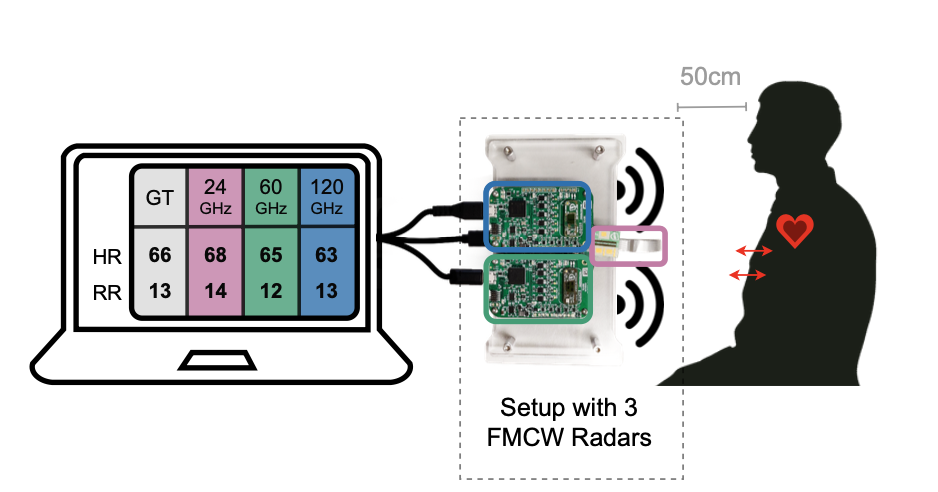
\includegraphics[width=0.7\linewidth]{Images/chapter3/3-1.png}
    \caption{ مقایسه تاثیر فرکانس روی اندازه گیری ضربان قلب \cite{marty2024frequency}.}
    \label{fig:fmcw_vitals}
\end{figure}